\documentclass{article}


\usepackage{polski}
\usepackage{indentfirst}
\usepackage{amsmath}
\usepackage{fancyhdr}
\usepackage{graphicx}
\usepackage{lipsum}
\usepackage{geometry}
\geometry{margin=1in}
\pagestyle{fancy}
\fancyhf{}
\rhead{Systemy wizualizacji procesów przemyslowych}
\rfoot{\thepage/\pageref{LastPage}}
\lfoot{Aleksander Orchowski}
\cfoot{\LaTeX}

\title{Systemy wizualizacji procesów przemysłowych}
\author{Aleksander Orchowski}
\date{}
\begin{document}
	\tableofcontents
	\section{Przedstaw podstawowe czynniki mające wpływ na powstanie klasy systemów	informatycznych określanych jako systemy SCADA.	}	
	\begin{itemize}
		\item Na zakładach produkcyjnych nieustannie wymuszana jest poprawa
		jakości wyrobu i lepsza organizacja produkcji. Jest to konsekwencja rosnącej
		konkurencyjność ma rynku oraz wprowadzenia nowych dyrektyw i ostrzejszych norm.
		\item Np. w zakładach przemysłu spożywczego od roku 1995 wdrażany jest
		jako standard HACCP (ang. Hazard Analysis and Critical Control Points ) i
		jego rozszerzona wersja ISO 22000:2005.		
		\item Różne inne normy (ISO 14001, 18001, 9001 itd.) dot. zarządzania jakością		
		\item  Potrzeba dostępu do historii wytwarzania wyrobu
		\item Wymóg poprawiania produktywności i poprawiania opłacalności produkcji
		\item Ograniczenie kosztów magazynowania
		\item Poprawa jakości wyrobów
		\item Możliwość analizy różnych czynników wpływających na produkcję, raportowanie, alarmowanie, monitorowanie i ułatwienie podejmowania decyzji oraz diagnostykę.		
		
	\end{itemize}
	

	
	\section{Przedstaw podstawowe funkcje systemów SCADA.}
	
	\begin{itemize}
	
	\item pomiar i przetwarzanie na jednostki fizyczne mierzonych wielkości;
	\item wizualizację procesu na ekranie synoptycznym (parametry, animacje);
	\item prezentację danych pomiarowych w postaci wykresów w funkcji czasu lub
	wykresów XY;
	\item kontrolę przekroczeń ograniczeń technologicznych i przekroczeń dopuszczalnej
	szybkości zmian parametrów;
	\item generowanie komunikatów alarmowych o awariach i przekroczenia parametrów
	technologicznych z podpowiedziami dla operatora;
	\item rejestrację alarmów i zdarzeń;
	\item wybór i zadawanie parametrów technologicznych;
	\item sterowanie automatyczne i zdalne węzłami technologicznymi;
	\item generator receptur umożliwiający tworzenie receptur i zarządzanie nimi;
	\item zapamiętanie i prezentowanie historii zmian (trendy bieżące i historyczne);
	\item archiwizację danych technologicznych;
	\item drukowanie bieżących raportów produkcyjnych;
	\item obróbkę statystyczną danych.
\end{itemize}
	
	
	
	
	\section{Scharakteryzuj część programową oraz sprzętową systemów SCADA.}
	\begin{itemize}
		\item Część sprzętowa
		  \subitem komputery PC
		  \subitem sterownik PLC lub/i kontrolery PAC,
		  \subitem panele operatorskie
		  \subitem aparatura pomiarowa (czujniki , przetworniki),
		  \subitem elementy wykonawcze (zawory, regulatory),
		  \subitem  urządzenia i okablowanie
		  \subitem sieci LAN oraz sieci przemysłowe		  
	    \item Część programowa
		  \subitem system operacyjny
		  \subitem oprogramowanie
		  \subitem narzędziowe do tworzenia aplikacji typu HMI/SCADA
		  \subitem programy komunikacyjne.		  
		\end{itemize}
	
	
\textbf{	część programowa systemów SCADA}


	Oprogramowanie SCADA funkcjonuje na określonym zestawie zmiennych (tagów, bramek, agentów), które są tworzone i edytowane przy użyciu programu zwanego konfiguratorem. Każda zmienna połączona jest ze slotem, w którym znajduje się opis do zmiennej. Pisanie oprogramowania rozpoczynamy od tworzenia ekranów synoptycznych (mimik , szablonów, templates), obrazów procesów technologicznych składających się z obiektów graficznych (wizardów), których zachowanie (behaviors) jest wcześniej zdefiniowane przez programistę. Stosuje się obiekty graficzne bierne i czynne. Te ostatnie połączone są zmiennymi, aby np. ruszały się na ekranie synoptycznym.
	
	\textbf{ Scharakteryzuj część sprzętową systemów SCADA. }
	
	Sterowniki (PLC lub PAC) pełnia rolę interfejsu między systemem informatycznym (SCADA) zainstalowanym w PC a sygnałami z urządzeń automatyki przemysłowej. Sterowniki PLC za pomocą odpowiednich interfejsów komunikacyjnych (moduły komunikacyjne), przy wykorzystaniu dedykowanych do zastosowań w obszarze przemysłu protokołów komunikacyjnych (sieci przemysłowe) zapewniają wymianę danych pomiędzy stacją kontrolo-nadzorczą (PC) a umieszczonymi w obiekcie sterownikami będącymi abonentami tej sieci. Najczęściej oprogramowania do modułów komunikacyjnych w sterownikach dostarczają mechanizmów pozwalających na odczyt i zapis danych z poszczególnych urządzeń. 
	\section{Przedstaw powiązanie systemu SCADA z obiektem sterowania, urządzeniami pomiarowo-sterującymi oraz innymi systemami informatycznymi w przedsiębiorstwie w ujęciu hierarchicznym i zarazem rozproszonym (rys).}
	\begin{figure}[!htb]
		\centering
		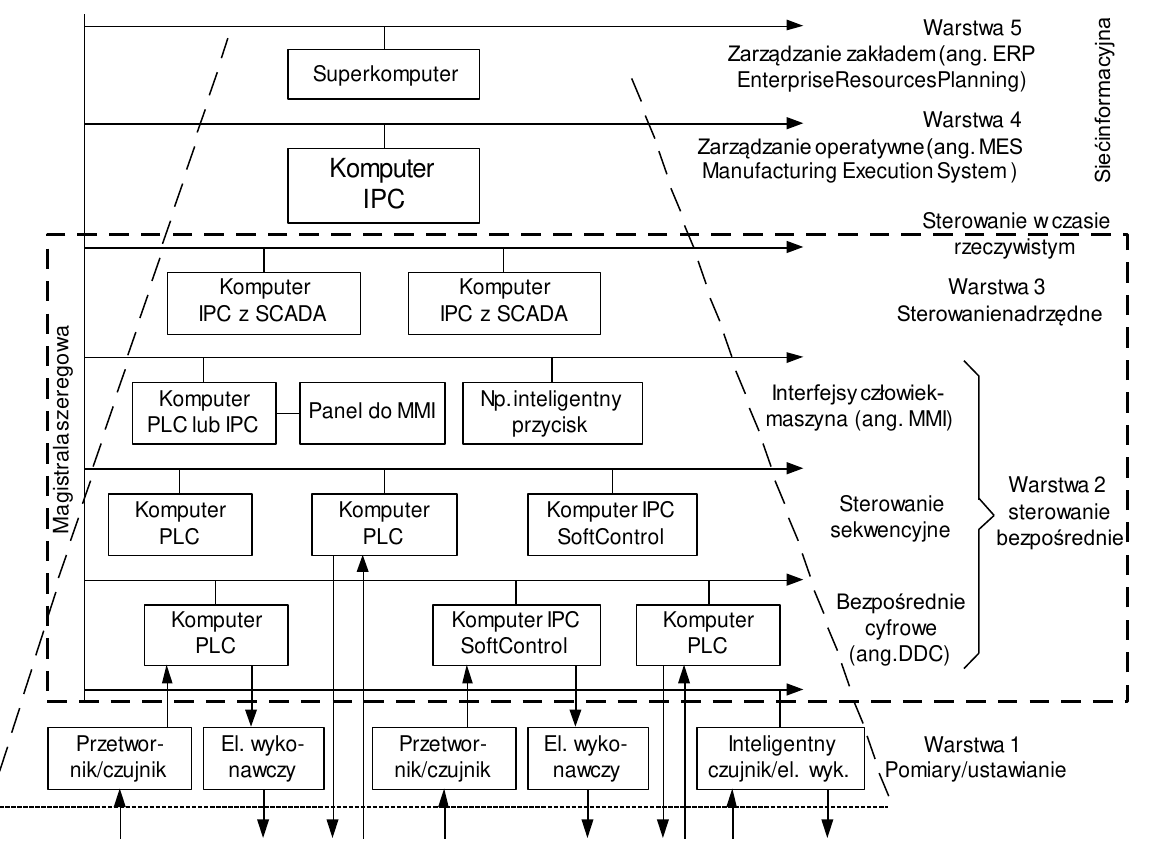
\includegraphics[width=1\linewidth]{schemat-obiekt-scada}
		\caption{tu coś trzeba naściemniać TODO}
		\label{fig:schemat-obiekt-scada}
	\end{figure}
	\section{Omów klasy oprogramowania wykorzystywane na poszczególnych poziomach	informatycznej struktury systemów przemysłowych.}
	\begin{figure}[!htb]
		\centering
		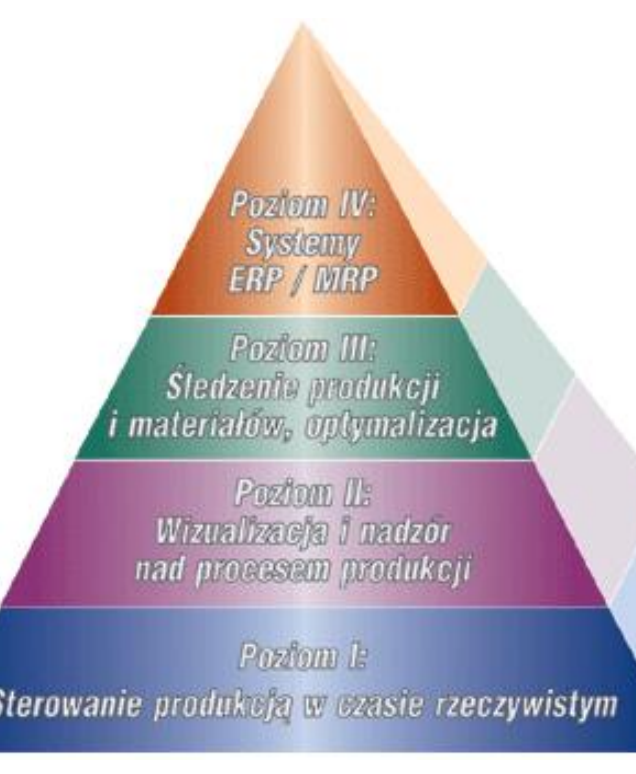
\includegraphics[width=0.3\linewidth]{piramida-fabryka}
		\caption{Warstwy oprogramowania w systemach przemysłowych.}
		\label{fig:piramida-fabryka}
	\end{figure}
	
	\subsection{POZIOM I: STEROWANIE PRODUKCJĄ W CZASIE RZECZYWISTYM}
	\begin{itemize}
		\item Stanowi pomost pomiędzy człowiekiem a maszynami i urządzeniami
		technologicznymi.
		\item Wykonuje procedury bezpośredniego sterowania poszczególnymi
		urządzeniami ciągu technologicznego.
		\item W ramach tego poziomu są również realizowane systemy monitoringu zużycia
		nośników energii oraz emisji zanieczyszczeń.
		\item Automatyzacja procesu produkcji na tym poziomie pozwala na podniesienie
		jakości wytwarzanego wyrobu poprzez ścisłe zachowanie parametrów procesu
		i racjonalizację zużycia energii.	
	\end{itemize}
    	\subsection{POZIOM II: WIZUALIZACJA I NADZÓR NAD PROCESEM PRODUKCJI.}
    	Podstawowe funkcje tego poziomu to funkcje systemów SCADA
    \begin{itemize}
    	\item Do poziomu II zaliczamy także systemy optymalizacji pracy urządzeń
    	technologicznych. Ich stosowanie pozwala na dalszą poprawę jakości
    	wytworzonego wyrobu oraz zmniejszenie zużycia energii i surowców
    	poprzez optymalizację prowadzenia procesu produkcyjnego.
    	\item Dzięki kontroli pracy całego ciągu technologicznego systemy poziomu II
    	dają możliwość generowania raportów z danymi na temat stanów urządzeń
    	i parametrów sterowania procesem.
    	\item  Przede wszystkim jednak dostarczają one interfejsu pomiędzy urządzeniem
    	a człowiekiem (MMI - Man Machine Interface ).    	
    \end{itemize}
    	Poziom II wiąże się ściśle z poziomem I, a ich funkcje często się przeplatają.
    	
    	\subsection{POZIOM III: ŚLEDZENIE PRODUKCJI I MATERIAŁÓW, OPTYMALIZACJA PROCESU}
	Poziom ten jest odpowiedzialny za wymianę danych pomiędzy systemami poziomów I i II, a
	systemami klasy ERP. Często po wprowadzeniu przejmuje on funkcje związane ze śledzeniem i
	dokumentacją procesu z poziomów I i II. Jednak do jego głównych zadań należy:
	\begin{itemize}
        \item modelowanie procesu produkcji;
        \item monitorowanie przepływu materiałów i środków produkcji w przedsiębiorstwie;
        \item wizualizacja i nadzorowanie produkcji;
        \item odczyt i archiwizowanie danych dotyczących procesu (produkcji);
        \item zarządzanie jakością;
        \item tworzenie dokumentacji produkcji;
        \item dynamiczne kierowanie ruchem zakładu;
        \item generowanie raportów;
        \item wprowadzanie i egzekwowanie właściwych praktyk produkcyjnych 
    	\end{itemize}
    Dzięki bezpośredniemu powiązaniu z systemami niższych poziomów proces ten przebiega dynamicznie, a
    stworzone plany produkcyjne mogą być modyfikowane na bieżąco w zależności od zaistniałych okoliczności.
    Pozwala to na reagowanie na takie zjawiska, jak nagłe zmiany zamówień spowodowane np. niespodziewanym
    załamaniem się rynku zbytu, poważne awarie urządzeń, braki lub niedobór zapasów surowców i półfabrykatów,
    zmiany priorytetów produkcji, itd.Podejście terytorialne zakłada, że każdy z ekranów
    synoptycznych systemu wizualizacji dostarcza informacji o
    urządzeniu (lub grupie urządzeń) zlokalizowanych w jednym miejscu
    instalacji i nadzorowanych przez jeden sterownik (lub grupę
    sterowników) przemysłowy.
    Zaleta: ograniczanie transferu informacji o stanie zmiennych przez
    sieci przemysłowe i dostosowanie scenariusza wymian sieciowych do
    wymagań aktualnie prezentowanego ekranu graficznego.
    
       \subsection{POZIOM IV: SYSTEMY ERP LUB MRP}
       	
       	\begin{itemize}
       	\item Systemy te zapewniają zwykle zarządzanie zasobami przedsiębiorstwa,
       	zamówieniami, zakupami, finansami, księgowością, kosztorysowaniem,
       	prognozowaniem i planowaniem jego działalności. Udostępniają bardzo często
       	narzędzia do optymalizacji procesu produkcji pod kątem kosztów lub
       	zapewnienia jakości.
       	\item Obejmują tzw. systemy biurowe przedsiębiorstwa, które nie są bezpośrednio
       	związane z produkcją, ale stanowią zaplecze logistyczne dla funkcjonowania
       	wydziałów produkcyjnych.
       	       	\end{itemize}5
       	Należy pamiętać, że granice pomiędzy poszczególnymi warstwami są czysto
       	umowne i zależnie od implementacji systemu dana funkcjonalność może być
       	realizowana na różnych poziomach.
       	
	\section{Przedstaw strukturę systemu wizualizacji z wykorzystaniem przemysłowych baz	danych.}
	\begin{figure}[!htb]
		\centering
		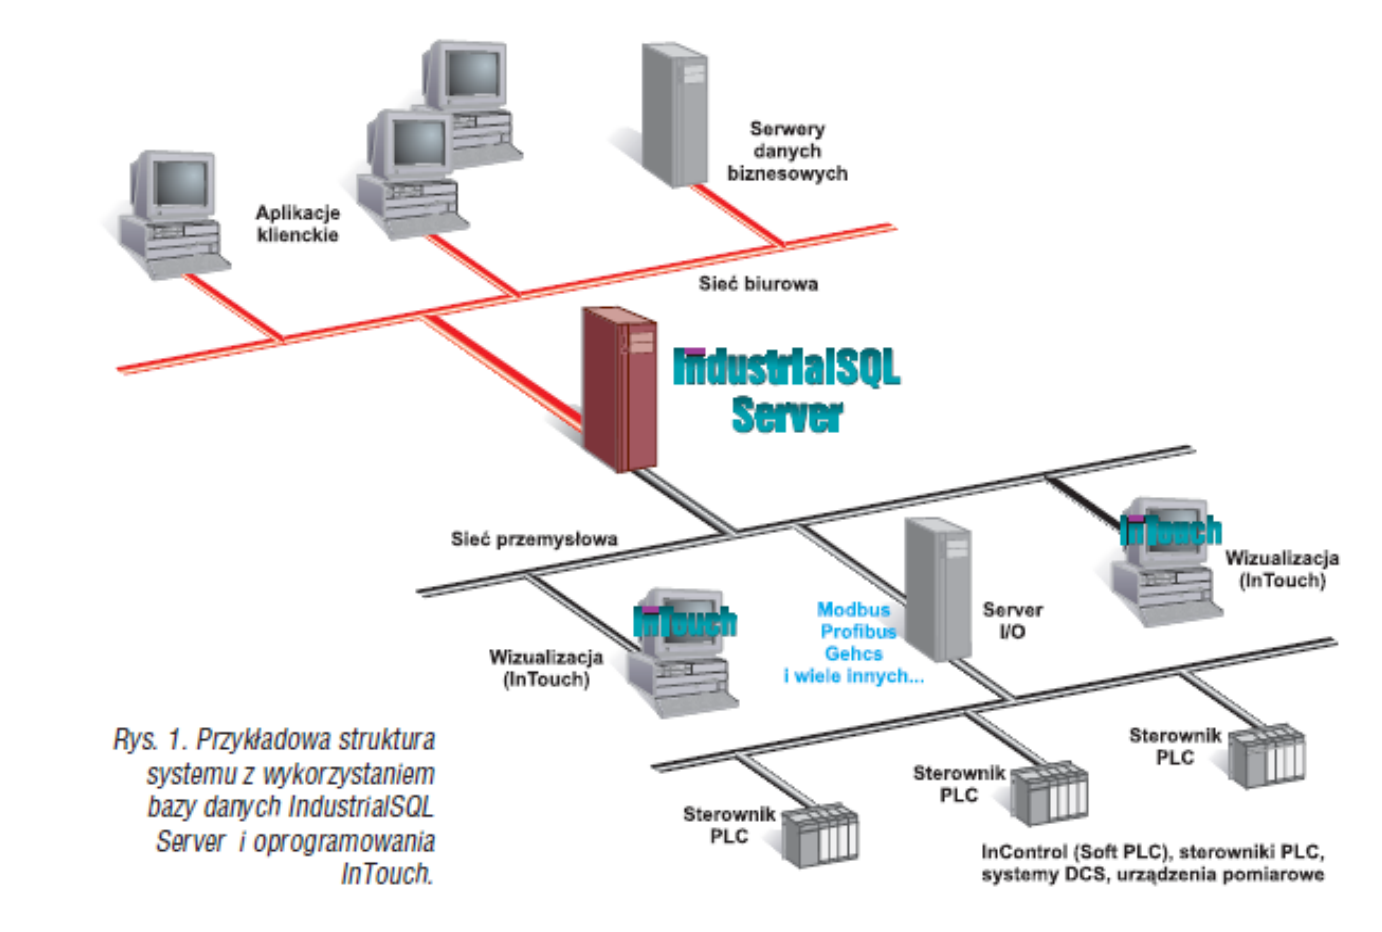
\includegraphics[width=0.7\linewidth]{industrialSQL}
		\caption{schemat}
		\label{fig:industrialsql}
	\end{figure}
	
	\begin{itemize}
		\item IndustrialSQL Server jest rozszerzeniem Microsoft SQL Serwera, który został wzbogacony o odpowiednie mechanizmy pobierania danych z PLCbuforowania ich, przechowywania i efektywnego ich odczytywania.
	
		\item Jest uzupełnieniem aplikacji wizualizacyjnych.
	
		\item IndustrialSQL Server zbiera informacje i rejestruje je w bazie danych, dostarczając automatykom i technologom bazy danych do tworzenia dowolnych raportów, zestawień, wykresów i analiz.
	
		\item Wraz z serwerem IndustrialSQL, który jest głównym elementem systemu, otrzymujemy kilka narzędzi klienckich do analizy danych.
	
		\item Dzięki pokrewieństwu IndustrialSQL Server z serwerem Microsoft SQL możliwa jest wymiana informacji z innymi systemami baz danych.
	
		\item IndustrialSQL Server bardzo dobrze współpracuje z oprogramowaniem InTouch, co jest naturalne, jako że stanowią elementy tego samego zintegrowanego pakietu dla przemysłu.
	
		\item Produkt ten można stosować wszędzie tam, gdzie dane pomiarowe, które chcemy rejestrować, dostępne są poprzez protokół DDE, OPC czy SuiteLink.
	\end{itemize}
	
	\section{Przedstaw podejście terytorialne i technologiczne stosowane podczas projektowania	ekranów synoptycznych systemów wizualizacji.}
	\textbf{Podejście terytorialne} zakłada, że każdy z ekranów
	synoptycznych systemu wizualizacji dostarcza informacji o
	urządzeniu (lub grupie urządzeń) zlokalizowanych w jednym miejscu
	instalacji i nadzorowanych przez jeden sterownik (lub grupę
	sterowników) przemysłowy.
	\textit{\textbf{Zaleta:}} ograniczanie transferu informacji o stanie zmiennych przez
	sieci przemysłowe i dostosowanie scenariusza wymian sieciowych do
	wymagań aktualnie prezentowanego ekranu graficznego.
	
	
	\textbf{Podejście technologiczne }zakłada grupowanie danych ze względu na
	ich powiązanie z określonymi fragmentami technologii. Informacje (np.
	parametry energetyczne z poszczególnych urządzeń) mogą pochodzić z
	różnych (często odległych) fragmentów instalacji. Ich grupowanie może być
	spowodowane nadzorowaniem nadrzędnym gospodarki energią na obszarze
	całego przedsiębiorstwa.
	\textbf{\textit{Rozproszenie terytorialne }}może znacznie komplikować pozyskiwanie
	informacji i ich przesyłanie w sieciach przemysłowych a także ich bieżące
	dostosowanie do potrzeb aktualnie prezentowanego ekranu graficznego.
	
	\section{Przedstaw podejście hierarchiczne stosowane podczas projektowania systemów	ekranów synoptycznych systemów wizualizacji.}
	Podejście hierarchicznego podziału ekranów graficznych wykorzystuje metodę kolejnych przybliżeń, gdzie stopniowo – w zależności od bieżących potrzeb – operator może przejść od ekranu prezentującego informacje ogólne (o największym poziomie agregacji) do najbardziej szczegółowych ekranów danego procesu (obiektu) – wycinka kontrolowanej instalacji technologicznej.
	
	Projektowanie hierarchiczne zakłada umieszczenie na ekranie głównym symbolicznego opisu całego obiektu. Stan poszczególnych podprocesów jest prezentowany na niej w sposób syntetyczny poprzez atrybuty związane z poszczególnymi urządzeniami i zespołami urządzeń.
	
	\section{Przedstaw proces (procedurę) projektowania systemu wizualizacji (diagram).}
	\section{ Przedstaw zalety i wady stosowania paneli operatorskich w systemach wizualizacji.}
	\section{ Omów budowę sterownika PLC w postaci kompaktowej i modułowej.}
	\textbf{Sterowniki  Kompaktowe}
	
	\begin{itemize}
	
	\item Konstrukcja kompaktowa  zawiera w sobie kompletny sterownik, składający się z CPU, zasilacza, modułu wejść/wyjść i modułu łącza szeregowego.
	
	\item Tego typu konstrukcja stosowana jest przeważnie do budowy sterowników małych.
	
	\item Zaletą jej jest prosta konstrukcja i łatwy montaż.
	
	\item Tego typu sterowniki posiadają możliwość rozbudowy. Realizowane jest to poprzez dołączenie dodatkowego bloku rozszerzającego, w którym znajdują się dodatkowe układy wejść/wyjść.
	
	\end{itemize}
	
	\textbf{Sterowniki Modułowe}
	
	\begin{itemize}
		
	\item Konstrukcja modułowa jest przeznaczona do zastosowań gdzie użytkownik sam dobiera konfiguracje sterownika.
	
	\item Umieszcza on w specjalnej obudowie poszczególne panele z modułami funkcjonalnymi, takimi jak: jednostka centralna, pamięci czy moduły wejść/wyjść.
	
	\item Konstrukcja panelowa stosowana jest głównie do sterowników średnich i dużych. Rozbudowa sterownika realizowana jest poprzez dodanie dodatkowej obudowy, gdzie można umieszczać układy wejścia/wyjścia.
	
	\end{itemize}
	
	\section{ Przedstaw budowę CPU sterownika PLC.}
	
	Budowa sterownika
	
	Sterowniki PLC są to komputery przemysłowe, które umożliwiają sterowanie pracą maszyn i urządzeń (w układzie otwartym i/lub zamkniętym). Maja one architekturę klasycznego komputera, na którą składają się:
	
	\begin{itemize}
		
	\item jednostka centralna CPU (ang. Central Processing Unit) wraz z pamięcią;
	
	\item moduły wejściowe i wyjściowe, przy użyciu których dochodzi do wymiany danych pomiędzy otoczeniem i komputerem.
	
	\end{itemize}
	
	\begin{figure}[!htb]
		\centering
		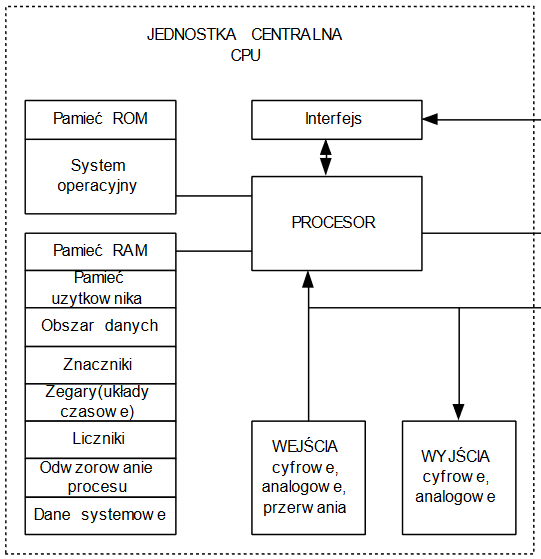
\includegraphics[width=0.7\linewidth]{cpu}
		\caption{Schemat jednostki centralnej}
		\label{fig:cpu}
	\end{figure}
	
	Jednostka centralna zawiera wewnątrz:
	
	\begin{itemize}
		
	\item procesor - prawie wszystkie sterowniki znajdujące się na rynku bazują na procesorach 16-bitowych, stąd słowo w sterownikach jest 16-bitowe, a wejście analogowe o rozdzielczości 10 lub 12 bitów zajmuje kanał 16 bitowy;
	
	\item pamięć operacyjną (ROM ang. Read-Only Memory) - trwałą pamięć, w której znajduje się system operacyjny (program systemowy, oprogramowanie systemowe) czyli zestaw programów sterujących i zarządzających działaniem sterownika (komunikacja z programistą, obsługa urządzeń zewnętrznych, zarządzanie danymi itd.), a także ostatnio pamięć bloków funkcji, parametry (ang. set-up) sterownika są w pamięci flash;
	
	\item pamięć programu (RAM ang. Random Access Memory) - zapisywalna pamięć podtrzymywana bateryjnie w której znajdują się obszary:·programu użytkownika w kilokrokach (kS), rzędu 5..30 kS, ale w dużych sterownikach do 400 kS, często składający się z kilku zadań, dawniej w zbliżonych jednostkach (kW),
	
	· danych sterownika,
	
	· danych systemowych,
	
	· danych o zegarach, licznikach, znacznikach,
	
	· odwzorowania procesu, czyli obrazu wejść i wyjść,
	
	· danych dla urządzeń zewnętrznych
	
	. Wszystkie te dane umieszczone są w pamięci danych rzędu 30 kW, choć w dużych sterownikach do 500 kW.
	
	\item moduły z wejściami/wyjściami cyfrowymi lub/i analogowymi albo moduły komunikacyjne (ang. Inner Board) –coraz częściej znajdują się w jednostkach centralnych.
	
	\end{itemize}
	
\label{LastPage}
\end{document}